\chapter{Introduction}
	\label{cha:intro}

	The mobile network has become an integral part of our everyday life.
	Internet access on the go serves us in a different way every minute; we use it to find someone, to translate foreign languages, to make ourselves or others laugh, to share memories, to reconnect to old friends or to create new ones.
	We use the mobile network to connect with each other.
	
	The human need to stay connected everywhere is seemingly endless, increasing the consumer use of mobile data year-by-year with a steady rate.
	This constantly increasing demand spurred the innovations in the \ac{5G} towards the use of capacity-increasing technologies on the radio link. 
	Most notable are the utilization of millimeter-wave carrier frequencies and spatial densification of the radio network using beamforming, massive \ac{MIMO} and micro- or pico-cells, achieving high peak data rates dubbed as \ac{eMBB}.
	These are the technological advancements that impact most of the consumers in \ac{5G}.
	However, \ac{5G} also pays attention to aspects of the network other than pure capacity; strict requirements towards high reliability, low latency or low battery consumption are also supported, allowing for uses of the network outside of the consumer sector (Fig.~\ref{fig:5g_feature_triangle}).
	
	\begin{figure}[ht]
		\centering
		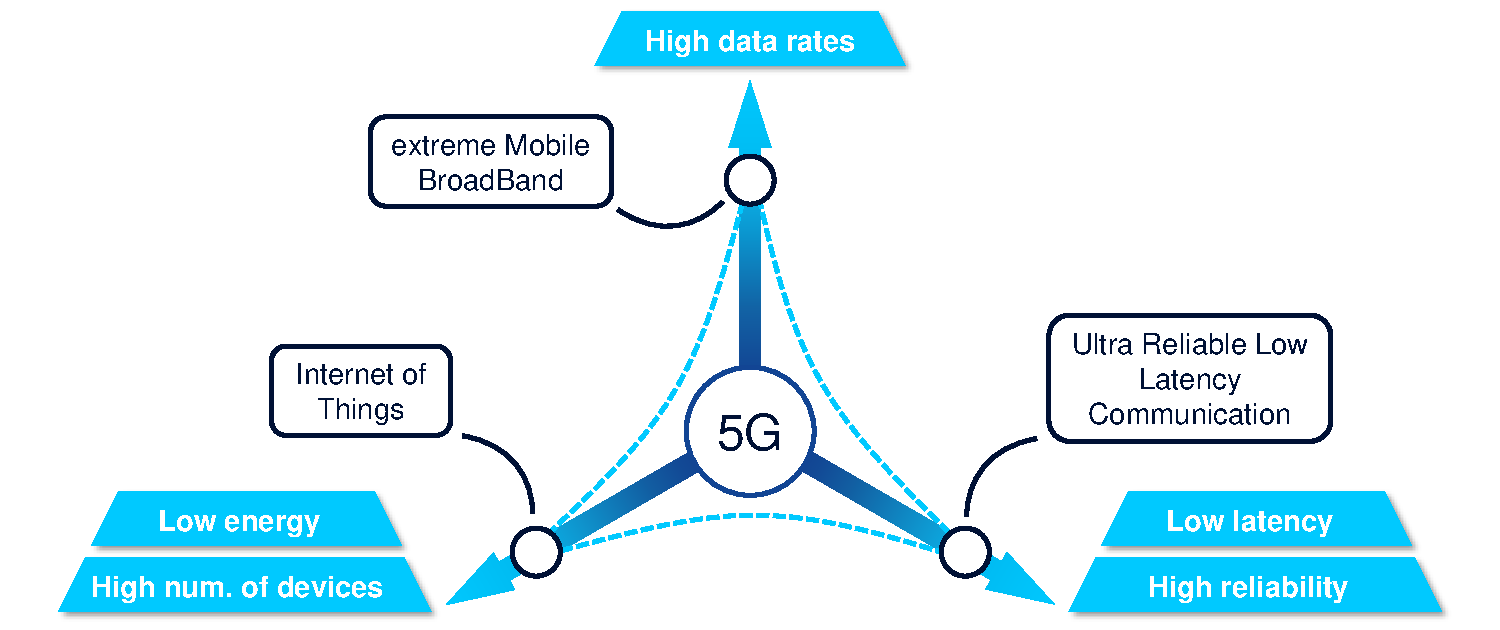
\includegraphics[width=\linewidth]{figures/01_introduction/5g_feature_triangle/5g_feature_triangle.pdf}
		\caption[Use cases with extreme requirements supported by 5G]{Use cases with extreme requirements supported by 5G.}
		\label{fig:5g_feature_triangle}
	\end{figure}
	
	A clear focus of \ac{5G} is the industrial applicability of mobile communication in use cases such as industrial sensor networks supported by low-energy \ac{IoT} features, or the remote control of machines in smart factories supported by \ac{URLLC} \cite{ngmn_5g_white_paper}.
	For now, these envisioned uses are still somewhat limited in their overall effect on the global mobile communication scene: industrial applications are mostly meant for isolated campus networks, and do not involve the generic consumer.	
	Moving beyond \ac{5G}, this constraint is lifting, with the use cases of the future requiring the widespread availability of reliable, low-latency and high-bandwidth communication.	
	If future mobile networks can achieve these requirements, life-changing improvements are possible in the commercial domains such as \cite{5g+_discussion_paper}:
	\begin{itemize}
		\item
			\textbf{Mobility:}
			Vehicles would be able to communicate with each other or the infrastructure, allowing for vastly improved traffic flow, remote control or on-demand autonomous driving without expensive equipment in the vehicles.
			
		\item
			\textbf{Healthcare:} 
			Connectivity-enabled devices and sensors would allow for the remote monitoring of patients, while \ac{AI}-based automated diagnosis will provide precise, real-time recommendations and warnings, improving survivability for many of the modern age's most deadly illnesses.
			
		\item
			\textbf{Retail:}
			The use of network-connected drones, as well as cashierless stores would allow for the time-efficient and personalized distribution of wares to the customers, while also simplifying and automating inventory management and warehouse operations.
	\end{itemize}
	
	By achieving these goals, the mobile network of the future could become even more deeply ingrained in our lives, with key moments not only supported by-, but depending on its functions.
	However, in order to support this vision, the mobile network of the future needs to be dependable.
	To be able to live up to these expectations, mobile networks not only need to support the connectivity requirements, but also need to be adaptive, robust, scalable and efficient.
	Furthermore, to be economically viable as a world-wide deployment, they also need to be cost-effective.
	Thus, the challenge is to create, setup, and maintain such a powerful network, which seems impossible without the use of automation that is close to- or even beyond human intelligence:
	cognitive autonomy.

	\section{Cognitive Autonomy}
	
		\subsection{Cognitive Autonomous Networks}
		
			There are key technological advancements that form the basis of the services in \ac{5G} and beyond: beamforming, massive \ac{MIMO} and millimeter-wave carrier frequencies in the radio access network, \ac{NFV} and \ac{SDN} in the core, with network slicing managing and distributing resources.	
			These technologies enable a network-scape that is vastly different from the traditional mobile network, with greatly increased density, heterogeneity, and elasticity.
			These aspects all contribute to a complex network scenario, which demands more than what the currently established network automation techniques are capable of.			
			In such complex networks, both the volume and variety of information that needs to be taken into account rules out traditional, hard-coded implementations.
			The possible contexts and environmental effects are too many, creating a vast state-space, which can no longer be effectively anticipated at design time.
			Furthermore, the effects that the different network elements have on each other also comes into play, where the interconnected nature of the network functions easily create conflicts.
			
			A modern solution to overcome the problem of enormous design-time complexity are learning algorithms, commonly referred to as \emphix{\ac{ML}}{machine!learning}.
			In \ac{ML} algorithms, the learning process creates a model using training data, by autonomously deducting rules which achieve the desired functionality.
			The use of \ac{ML} algorithms as a basis for network automation functionality enables $2$ major features:
			\begin{enumerate}[label=\textbf{\alph*})]
				\item \textbf{Autonomous deduction:}
					The description of the desired functionality is not done through explicit rules, but implicitly through supplying the learning algorithm with training data, which shows examples of correct functioning.
					This learning approach frees the designer of the function from having to create overtly complex rules, and allows for the design to focus more on describing the wanted behavior in a more efficient way.
					The designer's goal in this case becomes the extraction or generation of good quality training data for the algorithms, and the definition of fitting measures of goodness with which the \ac{ML} algorithms can be trained.
				
				\item \textbf{Continuous learning:}
					A natural step forward when using \ac{ML} algorithms is the notion of continuous learning.
					As the algorithms are already capable of deducting their own rules when training, this learning can be utilized during the operational phase to periodically or continuously update the model formed by the algorithm, making it able to adapt and optimize for changing environments.
					The task of the designer is to create methods that can extract good-quality training data on-the-fly while the algorithm is operational, as well as to create rules that govern the continuous training in order to balance adaptation against retainment of previously acquired knowledge.
			\end{enumerate}
		
			The \emphix{\ac{CAN}}{cognitive autonomous network} concept envisions just such a mobile network \cite{can_book}.
			In \ac{CAN}, cognitive entities, such as network management functions (\acp{CF}) take into account the context of their functioning in their recommendations or decisions.
			A cognitive entity is defined to be ``capable of perceiving a signal and process it into a data element, over which the entity reasons to select an action.
			It \emphnox{conceptualizes} and \emphnox{contextualizes} the data element and, logically or arithmetically [...] selects the appropriate action'' \cite{can_book}.	
			To be able to contextualize, the \acp{CF} must process large amounts of varied data, collected from many different parts and layers of the network.
			This increased receptive field is meant to enable a more insightful automation, one based on the comprehension of the interconnected dependencies/correlations in the network.
			However, cognition in \ac{CAN} also refers to a high cognitive power, where \acp{CF} are capable of automating tasks that require intelligence akin to human reasoning.
			Both the large receptive field and the high cognitive power mandates the use of \ac{ML} algorithms with a very strong modeling capability, which is only possible with the most complex, cutting-edge \ac{ML} algorithms today, most commonly known as deep learning.
			
		\subsection{The Cognitive Capabilities of Deep Learning}
			\label{cha:intro:sec:cognitive_cap_dl}
			
			\emphix{\ac{DL}}{deep learning} is a subset of machine learning, most commonly defined as \ac{ML} algorithms which utilize \acp{DNN} as their model (\ac{DL} is introduced in detail in Cha.~\ref{cha:deep_learning}).	
			Neural networks became the prime machine learning tool because of their capability to effectively select and utilize only the most important features from multi-dimensional input spaces containing low-level, raw features.
			Deep neural networks are capable of learning consecutively more abstract, higher-level latent representations from these low-level features during their training.
			The deeper the neural network, the stronger this abstraction can become, so much so that deep learning algorithms can effectively learn to do some of the same tasks that the human sensory system and brain can, in a single model, working on raw data.
						
			Deep learning algorithms are considered to be the most powerful machine learning tools to date.
			In some fields, such as \ac{NLP} or computer vision, deep learning algorithms allow for previously impossible tasks, such as precise machine translation of text, or self-driving cars.
			Deep learning algorithms are in fact so powerful in select applications, that they resemble human intelligence, and are often (confusingly) referred to as \ac{AI}.
			While my personal opinion is that current deep learning still has a long way to go before it can be called \ac{AI}, it is nevertheless important to see where exactly deep learning lies in cognitive power on the way to true \ac{AI}.
			
			For this, first we need to establish the distinction between the different \ac{ML} paradigms.			
			There are two major \ac{ML} paradigms: supervised learning and unsupervised learning.
			There exist various understandings and definitions of where the division lies between the two paradigms, but for the purpose of this discussion, I think it is best approached from the perspective of required human input:
			\begin{itemize}
				\item \emphix{Supervised learning:}{supervised learning}
					In this paradigm, the machine learning algorithm is trained on labeled training data.
					The labels are obtained through a laborious data preparation process before training, such as: manual labeling, directed feedback or measurement collection, or the setup of extensive simulated environments.	
					The labels are categorical or continuous values, and are attached to the training observations.
					The required output of the machine learning algorithm is the correct label for each input observation.
					The loss used for training the machine learning algorithm utilizes the labels as ground truth, and measures the difference between the output and the ground truth labels to steer the machine learning algorithm towards formulating the correct model.				
				
				\item \emphix{Unsupervised learning:}{unsupervised learning}
					In this paradigms, the machine learning algorithm is trained on unlabeled training data.
					Human labor is kept at a minimum in the data preparation process, generally requiring lightweight, easy-to-automate preparation before training, such as: data cleaning, feature- or temporal/spatial aggregation, or data segmentation.
					Human input is mostly relevant during design time, where the implementation of the additional constraints can embed some bias into the models formed by these algorithms.
					The required output of the machine learning algorithm is either the reconstruction or prediction of the input data itself, or some structure/logic that is found within the data.
					Unsupervised learning does not define the task explicitly in a way supervised learning does, instead defining it implicitly through additional constraints on the model, which the machine learning algorithm has to take into account during training.
					These additional constraints are often implemented as additional losses.					
	
			\end{itemize}		

			To correctly judge the cognitive capabilities of supervised and unsupervised deep learning algorithms, we can turn to a well known categorization of human cognitive processes: Bloom's taxonomy.			
			Proposed by the educational psychologist Benjamin Bloom at the University of Chicago in $1956$, the taxonomy is still widely used and updated \cite{bloom_taxonomy}. 
			Bloom's taxonomy organizes the different cognitive skills that students have to utilize during their studies, also referred to as learning objectives (Fig.~\ref{fig:bloom_taxonomy}).
			Simpler cognitive skills reside on the bottom of the taxonomy, while complex cognitive skills, which require high levels of intelligence and creativity, are towards the top.
			Similarly, the learning objectives these skills solve also go from concrete to abstract.
			We can look at the extremes to get a good grasp of the range of skills and estimate the requirements towards \ac{AI}.
			On the bottom, remembering is a very straight-forward task, one which was implemented long ago using memory in computers.
			At the top, creation, the unconstrained generation of things has so far been barely attempted with computers, where traditional software is usually only capable of handling situations which the programmer already thought of at design time, the very antithesis of creativity.
			\ac{ML} algorithms are a step in this direction, as they somewhat break this hard-codedness through their automatic model formulation.
			
			\begin{figure}[ht]
				\centering
				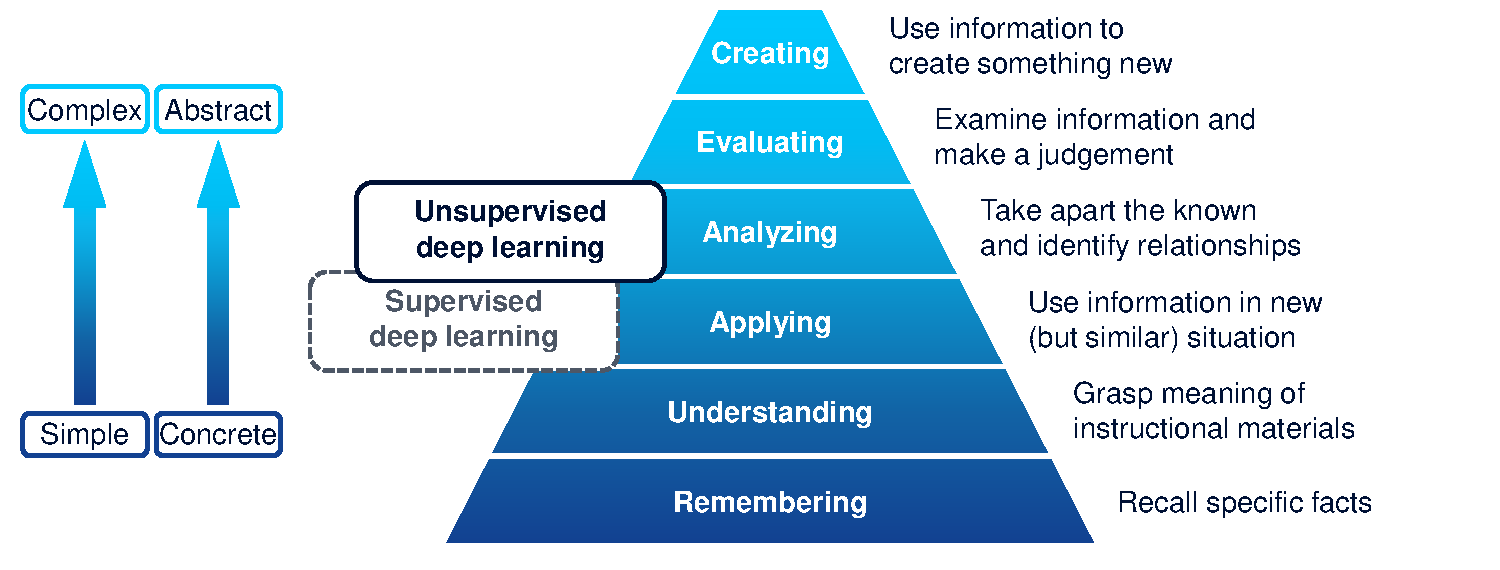
\includegraphics[width=\linewidth]{figures/01_introduction/bloom_taxonomy/bloom_taxonomy.pdf}
				\caption[Bloom’s taxonomy of cognitive learning processes]{Supervised and unsupervised DL positioned in Bloom’s taxonomy of cognitive learning processes.}
				\label{fig:bloom_taxonomy}
			\end{figure}
			
			Deep learning algorithms are a popular solution to tasks where the goal is to mimic human cognition in ordinary, everyday tasks.
			Computer vision problems such as object recognition, or image segmentation is something we do every minute, a large portion of our brains constantly dedicated to these tasks.
			\ac{NLP} problems, such as translating from one language to another is also a common task, one that some people use to communicate every day.
			These are problems where we humans have a very deep, intuitive understanding of the underlying logic, and even though we cannot effectively put the solutions of these problems into a set of simple rules, at least we can provide ample examples of solutions (labels), sufficiently covering all possibilities.
			Because these problems are solved everyday by all of us, researchers have access to large amounts of labeled training data through data mining labels on social media sites, or crowd-sourcing the labeling process.
			Thus, these tasks are best solved through \emphnox{supervised} learning, and so, most of the currently popular deep learning algorithms undertake this learning paradigm.
			Considering all this, I would position most current deep learning algorithms at the level of ``applying'' in Bloom's taxonomy: current \ac{DL} is very capable of remembering, understanding and applying complex rules that are derived from labeled examples generated by humans.
		
			Unfortunately, mobile networks do not have such label generation options.
			As network management tasks require expert knowledge, only a handful of people are capable of undertaking them.
			Furthermore, the tasks themselves are so complex that the required amount of labeled training data -- which would cover all possibilities -- is probably magnitudes larger than in the previously described everyday tasks.
			Requiring the handful of experts to manually generate that many examples for supervised learning is not feasible.
			Thus, for cognitive network automation, \emphnox{unsupervised} deep learning algorithms are of greater importance.
			Cognitive autonomous networks need \ac{DL} algorithms which can develop an understanding without explicit definition: \emphnox{analyzing} situations, or behavior by dissecting data and identifying relationships.
			This requires a higher level of cognition than what supervised \ac{DL} algorithms realize: analysis of information without specific patterns to detect is a more complex, and less concrete task than application of learned rules.
			In my opinion, such algorithms represent a higher level of cognitive power than supervised learning algorithms, occupying the ``analyzing'' slot on Bloom's taxonomy.
			I believe these algorithms represents progress towards true \ac{AI}, and are the future of \ac{DL} in the context of cognitive autonomous networks.
			
		 	I would like to mention a third machine learning paradigm here: \emphix{reinforcement}{reinforcement learning} learning.
			In reinforcement learning, the model learns by experimentation, through taking actions on an environment in order to maximize an often delayed reward.
			However, for mobile network automation, learning by experimentation is a complicated topic, because experimentation on large-scale, active network deployments is not feasible due to the many users depending on the mobile network's function.
			Furthermore, because of the large evaluation windows and slow reaction of the network to changes, such experimentation would possibly take a long time to converge.
			Therefore, in the mobile network context, reinforcement learning has to depend on simulated environments, which for network automation means complex digital twins that simulate many aspects of the network at the same time.
			Such detailed simulators were not available to us at the start of my research, and the topic itself is so vast, that it deserves its own dedicated researchers and multiple years of research. 
			Thus, this thesis focuses on algorithms that are unsupervised, but not on reinforcement learning, which is out of the scope of my research.
			
		\subsection{Gaps in Cognitive Network Automation Research}
			\label{cha:intro:sec:motivation}
		
			In my experience, much of the state-of-the-art research in mobile network automation focuses on realizing use cases with already available \ac{DL} algorithms.
			These algorithms are applied with little modification -- as a black box -- without tailoring or fine-tuning the algorithms to the specific use case.
			An in-depth overview of the uses of \ac{DL} in mobile networks is given in Sec.~\ref{cha:deep_learning:sec:related_work}.
		
			\ac{DL} is mostly advanced in other fields, such as computer vision and \ac{NLP}.
			Because the contexts and goals in these settings are very different from mobile network automation, the lack of dedicated research in our field can have long-term effects.
			As \ac{DL} algorithms become more and more performant, they also become ever more specific to the contexts they were developed for, which causes the performance in other applications to degrade.
			I believe that this specialization causes cutting-edge \ac{DL} algorithms to achieve lower performance in network automation tasks today, and will render them completely inapplicable in the long-term.
			An early sign of this trend is the already mentioned focus on supervised learning algorithms, which are of limited use in mobile network automation.
			
			Because of the lack of easily accessible labeling processes or labeled datasets, network automation aims to utilize semi- or unsupervised learning algorithms to be able to effectively learn from mobile network data.	
			These algorithms should be capable of autonomous analysis of data, without manually labeled datasets, or other types of extensive human supervision.
			However, unsupervised \ac{DL} algorithms are not prevalent, because the fields that progress \ac{DL} the most can utilize supervised learning algorithms better.
			Even if unsupervised \ac{DL} algorithms are developed, these will not necessarily be applicable to mobile networks, as unsupervised learning algorithms are especially prone to embed context-specific bias during design, in the form of additional constraints.
			
			Lastly, the lack of dedicated \ac{DL} research in mobile network automation could potentially result in unrealized use cases, for which there are no available \ac{DL} algorithms.
			I believe a side effect of dedicated research would be the invention of new \ac{DL} algorithms, which solve mobile-network-specific problems that do not exist in other fields.
			
			These observations motivated me to research unsupervised deep learning algorithms.
			My goal was to develop these algorithms specifically for mobile network automation, in order not to retain bias inherited from other technological fields, and to potentially enable new use cases that currently have no \ac{DL}-based solution.
			I have coined these algorithms as machine intuition.
		
	\section{Machine Intuition for Cognitive Network Automation}
	
		Human intuition is defined as ``the power or faculty of attaining direct knowledge or cognition without \emphnox{evident} rational thought and inference'' \cite{mw_intuition}.
		This definition does not mean intuition is insight gained without logic, from thin air: intuitive thinking certainly should infer knowledge from information using some form of reasoning.
		However, the reasoning might be quite abstract, as the derivation of the correct answer or structure from the data requires deep insight into latent features, which are hidden at first glance.
		While such cognition might seem to an outside observer as irrational, it should be possible to ground the insight in logical explanation, given that a wide enough scope of information is taken into account.
		
		To be considered as ``intuition'', a cognitive process must a) implement an unsupervised learning task, and b) require a deep insight into the data to uncover latent information.
		In order to further clarify intuition, I identified intuitive \emphix{processes}{machine!intuition!process}, which require the extraction of deep insight, achieved without external guidance, such as labeled observations.
		These intuitive processes are often used in conjunction with each other in problem-solving or communication.
		I have investigated $4$ such intuitive processes, which have potentially useful applications in mobile network automation:
		\begin{enumerate}[label=\textbf{\alph*})]
			\item
				\emphix{Exemplification}{exemplification} is the definition of a vocabulary of descriptive example observations, and the use of these examples to represent multiple observations, in order to effectively convey information in a dense, but easily understandable format.
			
			\item
				\emphix{Association}{association} refers to the extraction of important latent features in order to find meaningful similarities among the examples in the data, through which individual observations can be assigned to- and processed as discrete groups.
			
			\item
				\emphix{Prediction}{prediction} is the intelligent, long-term forecasting of future behavior of an entity, based strongly on contextual information such as historical data from the entity and/or similar entities, as well as information from the entity's surroundings.
			
			\item
				\emphix{Confidence}{confidence} refers to the treatment of incoming data and/or inferred information with uncertainty, and the communication of these doubts, in order to mitigate or completely stop the propagation of false information in automated processes.
		\end{enumerate}
		
		\emphix{Machine intuition}{machine!intuition} algorithms are \ac{DL} algorithms that realize the above cognitive processes.
		These algorithms are envisioned to be capable of in-depth analysis of varied, large-volume mobile network data through unsupervised learning.
		Lacking the need of extensive human supervision, machine intuition algorithms enable a network automation that is robust and adaptive, even when facing previously unforeseen situations.		
		By implementing these intuitive processes using \ac{DL} techniques, I also hoped to advance network automation to a higher level of cognition, where functions take into account a large scope for decisions, taking a step towards realizing the vision of \acp{CAN}.
			
	\section{Research Objectives and Thesis Outline}
	
		\subsection{Research Objectives}
		
			% Ox.1 Assess the feasibility
			% 	Q: Is it possible to realize this task using \ac{DL} algorithms?
			% Ox.2 Assess the applicability
			%	Q: In what way can these algorithms help? 	
			%	Q: Which tasks is it beneficial in, is it better than state-of-the-art?
			%	Q: Which use-cases might be enabled by this?	
			% Ox.3 Assess the practicality
			%	Q: Is it practical to use such algorithms in network automation tasks (runtime, data need, computation costs)?
			%
			% O5: Assess machine intuition as a whole in the context of cognitive network automation
			%	Q: Is deep learning truly the powerful tool everybody thinks it is for network automation
			%	Q: Do we need unsupervised learning, is it really not just a second best option to other learning paradigms?
			%	Q: Is machine intuition the correct tool to advance network automation towards a higher level of cognition?
			%	Q: Is it going to be ever adopted widely?

			The overarching research objective is to evaluate the concept of machine intuition applied for cognitive network automation tasks.
			To achieve this objective, the thesis explores the previously described $4$ machine intuition processes, by discussing a) implementations as \ac{DL} algorithms; b) the evaluation of these implementations with mobile network data; and c) possible applications in cognitive network automation tasks.
			My goal was to assesses $3$ aspects of each machine intuition process:
			\begin{enumerate}
				\item
					\textbf{Feasibility:}
					The first objective is establishing weather it is feasible to realize the machine intuition process with current \ac{DL} techniques.
					The answer might not be a simple yes or no: often, tasks can be solved using algorithms, but only with a certain accuracy, or only in specific circumstances.
					If so, the question is how precisely the process can be realized, and whether that precision is sufficient for the effective use in network automation.
									
				\item
					\textbf{Practicality:}
					The second objective is the assessment of the practicality of deploying such algorithms in a mobile network.
					As deep learning is a resource intensive undertaking, even if it is feasible, it might not be practical to use the algorithms, because the costs outweigh the benefits it provides to the network, and ultimately, to the users.
					Costs can include the need- and thus the overhead of communication of data, processing power, storage, or even the loss of privacy of the user.
					A major concern that can render an algorithm's use impractical is the training or inference time the algorithm needs, which usually scales with various parameters, such as input features, sequence lengths or number of network elements present in the data.
					While most of the algorithms discussed can be sped up with additional processing power, reaching a usable speed can render an algorithm impractical because of the extreme processing requirements.
					
				\item
					\textbf{Applicability:}
					The third objective is exploring which network automation tasks can be helped by the successful implementation of the machine intuition process.
					This assessment is often dependent on the feasibility and the practicality of the process; while some automation tasks can still leverage somewhat inaccurate or slow algorithms to their benefit, others have strict timing or precision requirements. 
					A further question is whether the realization of the intuitive process allows for new use cases.					
			\end{enumerate}
		
			Finally, I also intend to give a generic assessment on machine intuition as a whole, trying to answer whether unsupervised \ac{DL} is truly a tool to advance network automation, and whether it will enable more cognition for future mobile networks.
			With all this, the following are my research objectives, also summarized in Tab.~\ref{tab:res_objs}.
			
			\subsection*{A1: Assessment of Exemplification}
			
				Exemplification is discussed in the context of the automatic definition of network states.
				The network states are meant to be used as a ``vocabulary'', upon which communication can be based between cognitive functions in a \ac{CAN}.
				Exemplification should be realized by deep quantization algorithms, where a \ac{DNN} preprocesses data to extract the most descriptive features, which are then used by quantization algorithms to define the quantized states.
							
			\subsection*{A2: Assessment of Association}

				Association is examined in the context of cell and user clustering.
				Such clusters could be useful in classification-like tasks where labeled data is not available, such as user \ac{QoE} prediction, or in anomaly detection, detecting malfunctioning cells or malicious mobile users.
				Associative models should be realized by deep clustering algorithms, where a \ac{DNN} is tightly integrated with a clustering mechanism, enforcing the extraction of latent features with which groups become distinguishable in the data.
				
			\subsection*{A3: Assessment of Prediction}

				Prediction is evaluated in the context of user-specific dynamic radio control.
				By predicting the radio environment or user mobility in the long-term, preventative actions can be taken to avoid service outages -- such as triggering a handover -- increasing the reliability of the radio communication.
				Prediction should be implemented using sequence-processing-capable \acp{DNN}, where the temporal relationships in the data are taken into account in the models, either by specific filters, or through a memory present in the \ac{DNN}.
			
			\subsection*{A4: Assessment of Confidence}
			
				Confidence is discussed in the context of increasing robustness against erroneous data in \acp{CAN}, by communicating confidence values between \acp{CF}.
				Confidence values attached to data could allow \ac{DNN}-based \acp{CF} to learn to correct or disregard corrupted or malicious inputs, thereby increasing their dependability, and thus trust towards \acp{CAN}.
				The processing of confidence values should be integrated into the \acp{DNN} the \acp{CF} are based on, so that the \ac{DL} algorithms inherently learn to model tasks in a redundant way, and learn to use alternative inputs when others become corrupted.
			
			\subsection*{A5: Assessment of Machine Intuition}
			
				The final research objective is to give an overall assessment on the concept of machine intuition.
				This assessment is meant as a summary, where common aspects of machine intuition algorithms are discussed, in order to highlight the possibilities and potential caveats when using it in cognitive network automation.
				
			\begin{table*}[!h]
				\centering
				\renewcommand{\arraystretch}{1.2}
				\begin{tabular}{p{0.8\linewidth}}
					\textit{Assessment 1: Exemplification} \hfill Part \RomanNumeralCaps{1}\\
					\hline
					\hspace{4pt} A1.1: Feasibility of exemplification algorithms \\
					\hspace{4pt} A1.2: Practicality of exemplification algorithms \\
					\hspace{4pt} A1.3: Applicability of exemplification algorithms in CANs \\[12pt]
					
					\textit{Assessment 2: Association} \hfill Part \RomanNumeralCaps{2}\\
					\hline
					\hspace{4pt} A2.1: Feasibility of associative modeling \\					
					\hspace{4pt} A2.2: Practicality of associative modeling \\
					\hspace{4pt} A2.3: Applicability of associative modeling in CANs \\[12pt]
					
					\textit{Assessment 3: Prediction} \hfill Part \RomanNumeralCaps{3}\\
					\hline
					\hspace{4pt} A3.1: Feasibility of sequence prediction \\					
					\hspace{4pt} A3.2: Practicality of sequence prediction \\
					\hspace{4pt} A3.3: Applicability of sequence prediction in CANs \\[12pt]
					
					\textit{Assessment 4: Confidence} \hfill Part \RomanNumeralCaps{4}\\
					\hline
					\hspace{4pt} A4.1: Feasibility of machine confidence \\					
					\hspace{4pt} A4.2: Practicality of machine confidence \\
					\hspace{4pt} A4.3: Applicability of machine confidence in CANs \\[12pt]
					
					\textit{Assessment 5: Machine Intuition} \hfill Part \RomanNumeralCaps{5}\\
					\hline
					\hspace{4pt} A5.1: Increasing cognitive power for CAN \\
					\hspace{4pt} A5.2: Benefits/shortcomings of unsupervised DL \\
					\hspace{4pt} A5.3: Short- and long-term adoption, following trends \\						
				\end{tabular}
				\caption[Research goals]{Research goals in the context of thesis.}
				\label{tab:res_objs}
			\end{table*}				
			
%		\subsection{Approach}	
%
%			To be able to deduct general assessments for the research objectives, I have undertaken the following for one or more algorithms in each machine intuition subprocess:
%			\begin{enumerate}[label=\textbf{\alph*})]
%				\item
%					\textbf{Baseline research of \ac{DL} algorithm(s):}
%					I conducted baseline research on unsupervised deep learning algorithms, to realize functionality needed for machine intuition subprocesses.
%					These algorithms are mostly based on deep neural networks.
%					To implement machine intuition tasks with deep neural networks, either existing topologies, architectures or training techniques were to be modified, or completely new ones were to be invented.	
%				
%				\item
%					\textbf{Evaluation in the network automation context:}
%					In order to evaluate the algorithms, I aimed to utilize data either from real-world or simulated mobile network deployments.
%					Furthermore, I also aimed to evaluate other, similar algorithms in the same context, which meant re-implementation and re-evaluation of these algorithms on mobile network data, to be able to provide quantitative comparison of performance.
%								
%				\item
%					\textbf{(Optional) Contribution of findings to patents:}
%					I tried to contribute my findings to patents or standards, in order to influence the industry's approach in a direction that I think would make it possible to realize cognitive automation through machine intuition.
%			\end{enumerate}
%			
%			By undertaking the above steps, I hoped to gain insight in various \ac{DL} algorithms, network automation tasks and other mobile networks-related aspects of unsupervised \ac{DL}, with which I could provide assessments about the specific machine intuition subprocess.
		
		\subsection{Thesis Outline}
		
			In order to be able to present a cohesive discussion, first an overview of deep learning is given in Cha.~\ref{cha:deep_learning}.
		 	This background on \ac{DL} might be helpful for readers who are networking experts, but not necessarily experts in \ac{DL} techniques.
			At the end of this background chapter, a short high-level summary on the use of unsupervised \ac{DL} in mobile network automation is given.
		 	This related work section further emphasizes the observations made in Sec.~\ref{cha:intro:sec:motivation}.
		 	The current chapter on problem statement and research objectives, and the \ac{DL} background chapter together make up the (unnumbered) introductory part of the thesis.
		 	
			The rest of the thesis is organized into $4$ main parts, each corresponding to one of the $4$ main research objectives described previously (also highlighted in Tab.~\ref{tab:res_objs}).			
			Part \ref{part:exemplification} discusses exemplification, Part \ref{part:association} focuses on associative modeling, Part \ref{part:prediction} discusses sequence prediction, and Part \ref{part:confidence} evaluates the concept of machine confidence.			
			In these parts, each chapter discusses a research topic relevant for the machine intuition process, including the findings from one or more publications.
			The chapters are organized around singular topics and a main publication, with some chapters also discussing additional, supplementary publications.
			My contribution to each publication is detailed in the respective chapter introductions.
			The research objectives are summarized at the end of each part in a concluding chapter, highlighted with the ``Summary'' keyword in their title.
			Additionally, some sections discuss concepts taken from inventions/patent applications, which are highlighted with the ``Concept'' keyword in their title.
			While these concepts have no real scientific merit by themselves, they are sometimes important for the understanding of the bigger context of the research.					
			Part \ref{part:conclusion} concludes the thesis, corresponding to the fifth research objective.
			As closing notes, I also discuss my experiences with \ac{DL} research in mobile networks, as well as the current direction of patents and standardization regarding this topic.			
			
			This thesis discusses two types of networks: mobile networks and neural networks.
			In order to avoid confusion, mobile networks will be always referred to as ``networks'', while neural networks will be referred to with the shortened form, as ``nets''.
			The mobile networking field is plagued with an overuse of abbreviations.
			In an effort to combat this phenomenon, I provide a list of acronyms.
			Furthermore, some expressions might be unfamiliar to the reader.
			These expressions are highlighted with a \textbf{bold} lettering, and are collected in an index for easy lookup.
		
		\vfill
			
		\subsection{Publications in the Context of this Thesis}
			
			This thesis is based on the following peer-reviewed publications:
			
			\begin{publication}
				Equal-volume Quantization of Mobile Network Data using Bounding Spheres and Boxes \\
				\textit{Márton Kajó, Benedek Schultz, Janne Ali-Tolppa, Georg Carle} \\
				NOMS 2018-2018 IEEE/IFIP Network Operations and Management Symposium, pp. 1-9. IEEE, 2018.
			\end{publication}
			
			\begin{publication}
				Environment Modeling and Abstraction of Network States for Cognitive Functions \\
				\textit{Stephen S. Mwanje, Márton Kajó, Sayantini Majumdar, Georg Carle} \\
				NOMS 2020-2020 IEEE/IFIP Network Operations and Management Symposium, pp. 1-8. IEEE, 2020.
			\end{publication}
			
			\begin{publication}
				Deep Clustering of Mobile Network Data with Sparse Autoencoders \\
				\textit{Márton Kajó, Benedek Schultz, Georg Carle} \\
				NOMS 2020-2020 IEEE/IFIP Network Operations and Management Symposium, pp. 1-6. IEEE, 2020.
			\end{publication}
			
			\begin{publication}
				Mobility and QoS Prediction for Dynamic Coverage Optimization \\
				\textit{Janne Ali-Tolppa, Márton Kajó} \\
				NOMS 2020-2020 IEEE/IFIP Network Operations and Management Symposium, pp. 1-2. IEEE, 2020.
			\end{publication}
			
			\begin{publication}
				Modeling and Abstraction of Network and Environment States Using Deep Learning \\
				\textit{Stephen S. Mwanje, Márton Kajó, Janne Ali-Tolppa} \\
				IEEE Network 34, no. 6 (2020), pp. 8-13.
			\end{publication}
					
			\begin{publication}
				Neural Network-based Quantization for Network Automation \\
				\textit{Márton Kajó, Stephen S. Mwanje, Benedek Schultz, Georg Carle} \\
				arXiv preprint arXiv:2103.04764 (2021).
			\end{publication}
			
			\begin{publication}
				Machine-Learning-Based Predictive Handover \\
				\textit{Ahmed Masri, Teemu Veijalainen, Henrik Martikainen, Stephen S. Mwanje, Janne Ali-Tolppa, Márton Kajó} \\
				IM 2021-2021 IFIP/IEEE International Symposium on Integrated Network Management, pp. 1-2. IEEE, 2021.
			\end{publication}
			
			\begin{publication}
				Clustering Mobile Network Data with Decorrelating Adversarial Nets \\
				\textit{Márton Kajó, Janik Schnellbach, Stephen S. Mwanje, Georg Carle} \\
				NOMS 2022-2022 IEEE/IFIP Network Operations and Management Symposium, pp. 1-9. IEEE, 2022.
			\end{publication}
		
			\begin{publication}
				Robust Deep Learning against Corrupted Data in Cognitive Autonomous Networks \\
				\textit{Márton Kajó, Janik Schnellbach, Stephen S. Mwanje, Georg Carle} \\
				NOMS 2022-2022 IEEE/IFIP Network Operations and Management Symposium, pp. 1-7. IEEE, 2022.
			\end{publication}
			
			Additionally, the following \ac{CAN} book chapters (which I am a co-author of) are also mentioned \cite{can_book}:
			
			\begin{publication}
				Classic Artificial Intelligence: Tools for Autonomous Reasoning \\
				\textit{Stephen S. Mwanje, Márton Kajó, Benedek Schultz, Kimmo Hatonen, Ilaria Malanchini} \\
				Towards Cognitive Autonomous Networks: Network Management Automation for 5G and Beyond (2020): 173-201.
			\end{publication}
			
			\begin{publication}
				Machine Learning: Tools for End‐to‐End Cognition \\
				\textit{Stephen S. Mwanje, Márton Kajó, Benedek Schultz} \\
				Towards Cognitive Autonomous Networks: Network Management Automation for 5G and Beyond (2020): 203-254.
			\end{publication}
			
			\begin{publication}
				Cognitive Autonomy for Network Self‐Healing \\
				\textit{Janne Ali-Tolppa, Márton Kajó, Borislava Gajic, Ilaria Malanchini, Benedek Schultz, Qi Liao} \\
				Towards Cognitive Autonomous Networks: Network Management Automation for 5G and Beyond (2020): 345-384.
			\end{publication}
			
			Finally, this thesis also contains mentions of the following patent applications:
						
			\begin{patent}
				Diagnosis Knowledge Sharing for Self-healing \\
				\textit{Benedek Schultz, Janne Ali-Tolppa, Márton Kajó} \\
				WO, PCT application no.: PCT/EP2018/079735, filed Oktober 2018
			\end{patent}
			
			\begin{patent}
				Environment Modeling and Abstraction of Network States for Cognitive Functions \\
				\textit{Benedek Schultz, Márton Kajó, Stephen S. Mwanje} \\
				WO, PCT application no.: PCT/EP2018/069638, filed July 2018
			\end{patent}
			
			\begin{patent}
				Method and Apparatus for Automatic Network State Modeling in Mobile Networks using Deep Clustering Autoencoders \\
				\textit{Benedek Schultz, Márton Kajó, Stephen S. Mwanje} \\
				Finnish application no.: 20206162, filed November 2020
			\end{patent}
		
			\begin{patent}
				Latent Variable Decorrelation for Deep Clustering in Mobile Networks \\
				\textit{Janne Ali-Tolppa, Márton Kajó, Stephen S. Mwanje} \\
				WO, PCT application no.: PCT/EP2020/072019, filed August 2020
			\end{patent}
			
			\begin{patent}
				Path-Aware Cognitive Handover Optimization (PACHO) \\
				\textit{Janne Ali-Tolppa, Márton Kajó, Stephen S. Mwanje} \\
				WO, PCT application no.: PCT/EP2021/072325, filed August 2021
			\end{patent}
			
			\begin{patent}
				Accounting for Erroneous Data in Learning and Inference of Cognitive Functions through Confidence Indicators \\
				\textit{Anubhab Banerjee, Márton Kajó, Stephen S. Mwanje} \\
				WO, PCT application no.: PCT/EP2021/067609, filed June 2021
			\end{patent}
		

